\section{Durchführung}
\label{sec:Durchführung}

\subsection{Versuchsaufbau}
\label{subsec:Versuchsaufbau}
Der Versuchsaufbau ist in \autoref{fig:versuchsaufbau} zu finden.
Die Apparatur besteht hauptsächlich aus dem Geiger-Müller-Zählrohr (1), der Kupfer-Röntgenröhre (2)
und dem LiF-Kristall (3).
Ein angeschlossener Rechner nimmt dabei alle Werte auf.
Die Beschleunigungsspannung $U_B$ beträgt $\SI{35}{\kilo\volt}$ und der Emissionsstrom $I = \SI{1}{\milli\ampere}$.

\begin{figure}
    \centering
    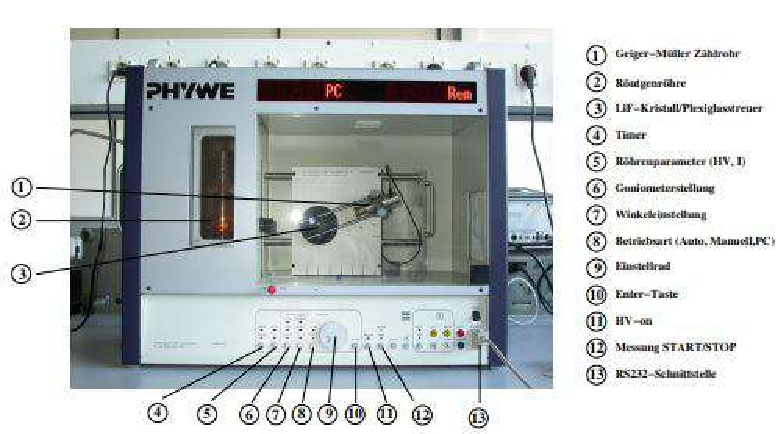
\includegraphics[width=\textwidth]{content/versuchsaufbau.pdf}
    \caption{Versuchsaufbau vor Ort.\cite{anleitung}}
    \label{fig:versuchsaufbau}
\end{figure}

\subsection{Überprüfung der Bragg-Bedingung}
\label{subsec:braggbedingung}
Der LiF-Kristall wird auf einen Winkel $\theta = 14°$ gestellt.
Das Geiger-Müller-Zählrohr wird zwischen $26° \leq \alpha_{GM} \leq 30°$ in $\increment \alpha_{GM} = 0.1°$ Schritten variiert.
Die Integrationszeit beträgt dabei $t = \SI{5}{\second}$.

\subsection{Analyse des Emissionsspektrums der Cu-Röntgenröhre}
\label{subsec:emissionspektrum}
In $\increment \theta = 0.1°$ Schritten wird das Emissionsspektrum im Winkelbereich $\SI{8}{\degree} - \SI{25}{\degree}$ über
 eine Integrationszeit von $t = \SI{10}{\second}$ aufgenommen.
Ein Detailspektrum der Kupfer $K_\alpha$  und $K_\beta$ Linien wird nicht aufgenommen.
Dies wird im 2:1 Koppelmodus durchgeführt.

\subsection{Analyse der Absorptionsspektren}
\label{subsec:absorptionsspektren}
Die verschiedenen Absorber werden zwischen dem LiF-Kristall und dem Geiger-Müller-Zählrohr gesetzt.
Die Integrationszeit beträgt $\SI{20}{\second}$ bei einem Winkelzuwachs von $\increment \theta = \SI{0.1}{\degree}$.
Die Winkelbereiche werden für jeden Absorber individuell gewählt.